\documentclass[11pt]{article}

\usepackage{fullpage}
\usepackage{url}
\usepackage{amsmath,amsthm,amssymb}
\usepackage{graphicx}		
\usepackage{setspace}
\usepackage[T1]{fontenc}
\usepackage{lmodern}
\usepackage{titling}
\usepackage{enumerate}
\usepackage{titlesec}
\usepackage{makeidx}

\titleformat{\section}
  {\normalfont\fontsize{12}{15}\bfseries}{\thesection}{1em}{}

\setlength{\droptitle}{-5em}   
\newcommand*{\TitleFont}{%
      \usefont{\encodingdefault}{\rmdefault}{n}{b}%
      \fontsize{14}{16}%
      \selectfont}
      

%\title{\TitleFont \textbf{Regression Models with Missing Data}}
%\author{\TitleFont Matteo Bonvini, Angela Fan}

\title{\TitleFont \textbf{SPU 22 Term Project Proposal}}
\author{\TitleFont Robbie Gibson}
\date{ }

\begin{document}
\maketitle

\vspace{-1.5cm}

\setlength{\parskip}{0.5em}

I would really like to make a web visualization to help people learn about the Earth.
Last year, I took CS 171: Visualization, which taught me how to create beautiful, interactive web visualizations, so I want to apply that to this class.
Just as an example, you can look at my final project for that class: D2Dota (\url{http://d2dota.com/}).
This was a project for three people, so what I could make for this class would be less, but it's a good overview of what is possible.
I really enjoyed that class, and I want to do my best to combine all my interests.
Also, I think that this would be a really cool interactive way to teach people cool science facts.

My vision would be to have two views of the Earth.
The first would be a globe view of the outside of the Earth.
There would be markers on the globe which, when selected expand to give stories of important times in the history of the study of the Earth or values of certain quantities.
For instance, there would be some marker which told the circumference of the Earth.
Another marker, in Egypt, would tell how Eratosthenes measured the Earth's circumference.
The second view would strip off the outer terrain and reveal the innards of the Earth.
Here, viewers could learn about the mantle and the two cores, as well as read how these were discovered.
As an example, one marker could mention the mass of the Earth and how that was discovered.
Another could talk about P and S waves and how they work.
Viewers could switch between the two views at will and investigate wherever they wanted.
The descriptions would appear in pop-ups over the Earth or on the side, and would hopefully contain links to websites with more information or sources.
Then, depending on how much work this all takes, I could perhaps add in more features.

I basically see the project as the beginnings of a museum exhibit.
It could theoretically appear on some display in a museum hall for visitors to interact with, although the end product here will be a website, or a least a web page.
Overall, I hope this could encourage people to learn more about their own home and the history behind discoveries about it.

Below is a quick example of what the site could look like, although it is very rough:

\begin{center}
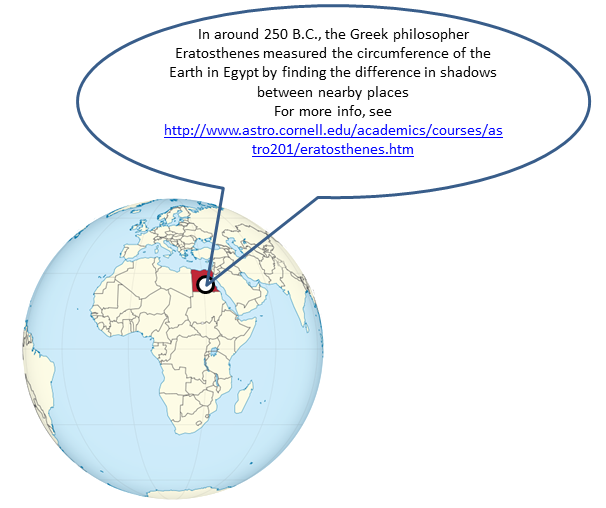
\includegraphics[scale=0.6]{projectpropimg.png}
\end{center}

\end{document}